%%***( Escalamiento del Sistema )***************************************************

A partir del sistema base modelado en PragmaDev Studio, se construye un nuevo sistema, que considera múltiples instancias de cada agente (proceso SDL).\\

%%==================================================================================
\section{Diagramas MSC}

A comparación de la primera versión de los diagramas MSC, durante la realización del proyecto se realizaron varias modificaciones para hacer un mejor diseño en la arquitectura del mismo. \\

El primer cambio es que ahora en vez de usar un diagrama general MSC se hicieron varios diagramas para mostrar todo el funcionamiento de una manera más organizada y correcta, para esto se separó el diagrama principal en 5 diagramas MSC. \\

Dentro de los diagramas, para  hacer la acción del movimiento, se utiliza el diagrama de la figura \ref{MoveMSCx} , el cual solo tiene un fragmento en caso de que el trigger de movimiento se active.

\begin{figure}[h]
    \centering
    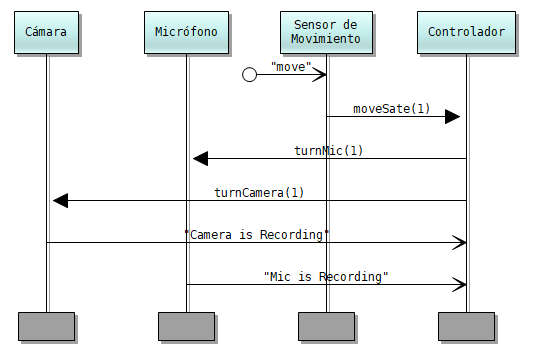
\includegraphics[width=0.5\textwidth]{images/Move_MSCx.png}
    \caption{Diagrama MSC cuando se registra un movimiento.}
    \label{MoveMSCx}
\end{figure}

\pagebreak

Lo mismo aplica en la figura \ref{NoMoveMSCx}, la cual muestra el mismo proceso pero cuando ya no se está movimiento algo en la zona registrada, además cuando se envía al controlador esta redirige la información al servidor y este envía la información para salvarla en la base de datos.

\begin{figure}[h]
    \centering
    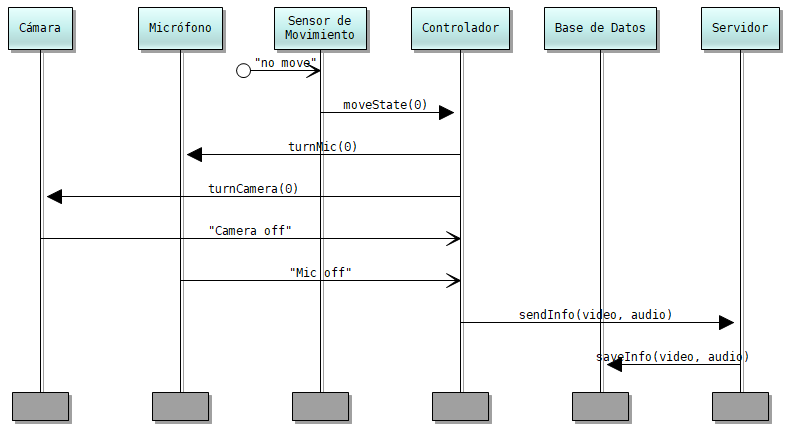
\includegraphics[width=0.8\textwidth]{images/NoMove_MSCx.png}
    \caption{Diagrama MSC cuando no se registra un movimiento.}
    \label{NoMoveMSCx}
\end{figure}

Cuando un usuario va a hacer un requerimiento, este presenta las mismas acciones que el modelo MSC original, como se puede ver en la figura \ref{RequestMSCx}.

\begin{figure}[h]
    \centering
    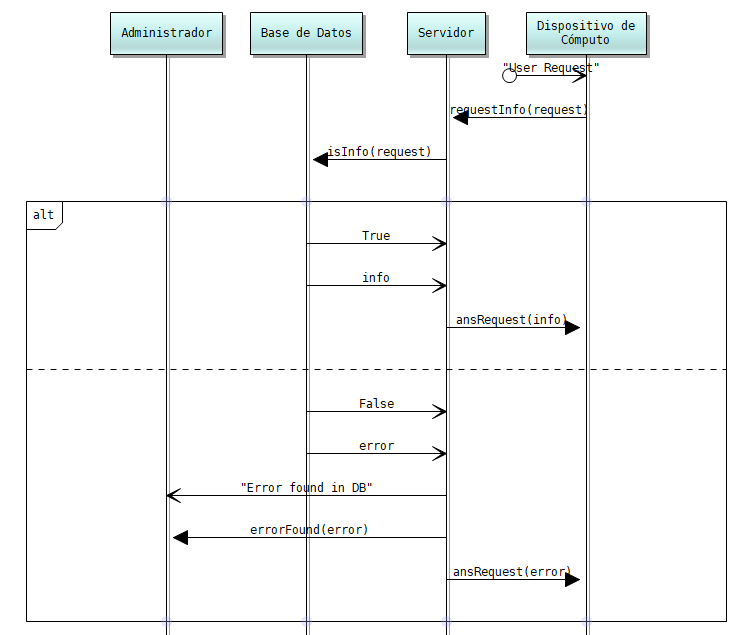
\includegraphics[width=0.58\textwidth]{images/UserRequest_MSCx.png}
    \caption{Diagrama MSC cuando se registra un requerimiento.}
    \label{RequestMSCx}
\end{figure}

\pagebreak

Al momento de que haya un problema en el sistema por parte de los dispositivos, que sería un evento importante y que se puede predecir, no cambió respecto al primer planteamiento del sistema, como se puede ver en la figura \ref{ProblemMSCx}.

\begin{figure}[h]
    \centering
    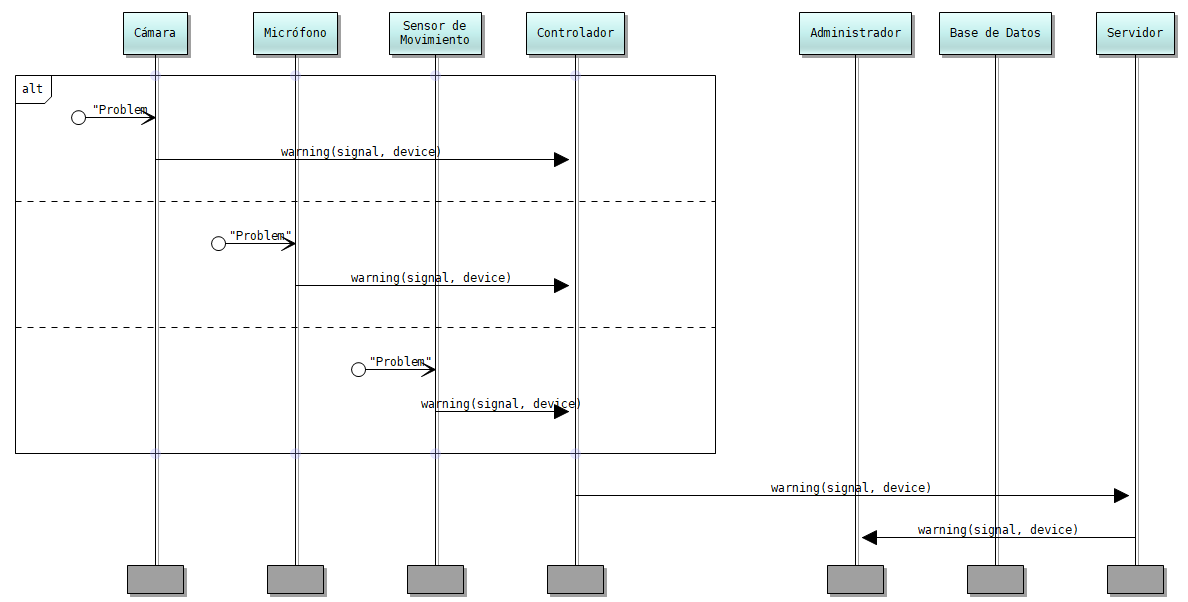
\includegraphics[width=0.9\textwidth]{images/Problem_MSCx.png}
    \caption{Diagrama MSC cuando se registra un problema en el sistema.}
    \label{ProblemMSCx}
\end{figure}

Por último, en la figura \ref{DropInfoMSC1} y en la figura noc2, está el caso en el que se elimina la información de la base de datos, esto permite que la información durante el periodo de investigación para los usuarios no se llena la base de datos y no se tenga que utilizar recursos, es por eso que se le envía al usuario un mensaje sobre la información que se eliminará para que descargue la información que necesita y una vez cumplido el tiempo para guardar la información (una semana aproximadamente) se elimina la información de la base de datos, para que el usuario o los siguientes usuarios puedan hacer uso nuevamente de la base de datos y esta no se llene ni tenga problemas porque base de datos se encuentra sin espacio.

\begin{figure}[h]
    \centering
    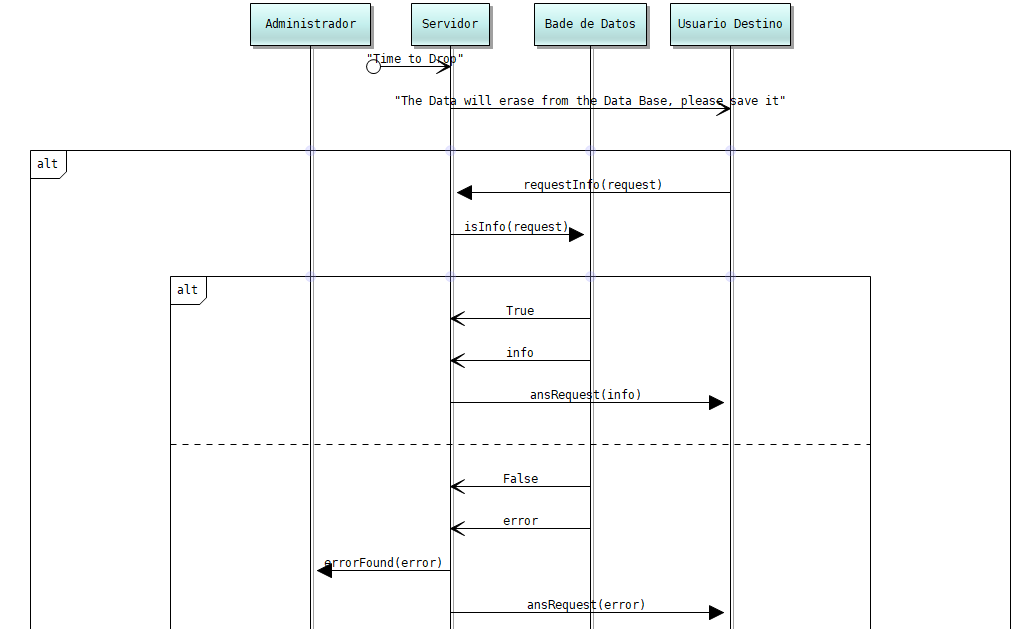
\includegraphics[width=0.7\textwidth]{images/DropInfo_MSC1x.png}
    \caption{Diagrama MSC cuando se va a eliminar la información (1/2).}
    \label{DropInfoMSC1}
\end{figure}

\pagebreak

Por un lado, si el usuario decide traer la información para guardarla localmente una vez le llega el mensaje sobre la información que será eliminada, este envía un requerimiento cuyo manejo ya se mostró anteriormente en la figura \ref{RequestMSCx}, para esto si el requerimiento es verdadero devuelve la información y si es falso devuelve un error tanto para el usuario como para el administrador en la figura \ref{DropInfoMSC2}

\begin{figure}[h]
    \centering
    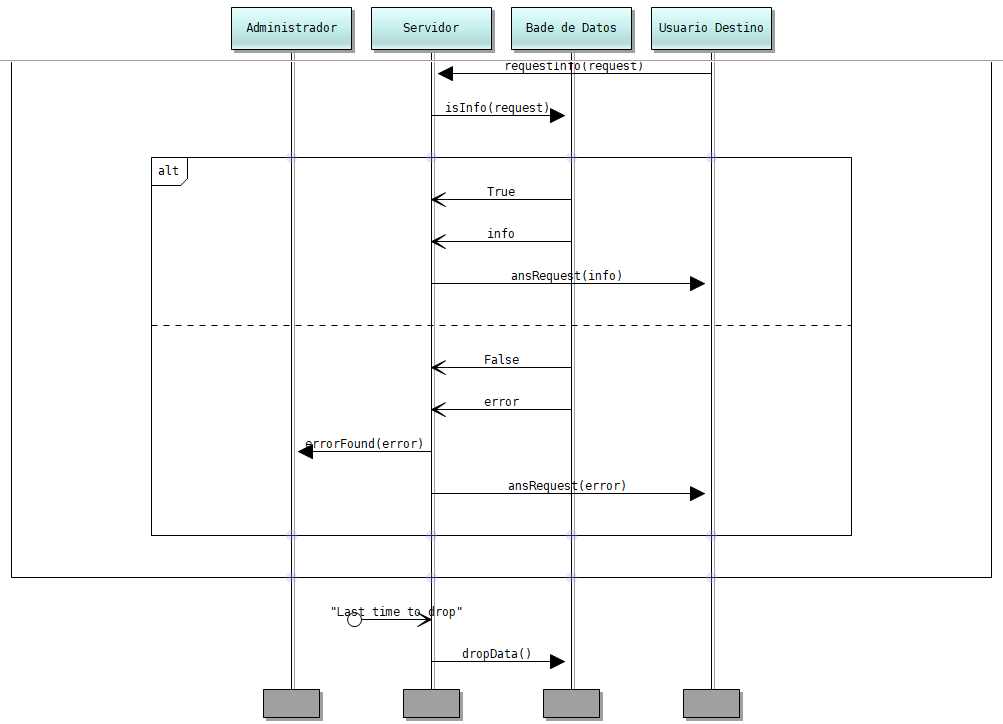
\includegraphics[width=0.65\textwidth]{images/DropInfo_MSC2x.png}
    \caption{Diagrama MSC cuando se va a eliminar la información (2/2).}
    \label{DropInfoMSC2}
\end{figure}

\pagebreak

%%==================================================================================
\section{Arquitectura SDL y procesos}

Incluya diagramas (PragmaDev Studio) con la arquitectura (estructura) del sistema escalado y de los respectivos procesos SDL (comportamiento).

Para la arquitectura SDL se hicieron varios cambios, principalmente fue quitar algunos procesos que no eran necesarios y solo se dejaron bloques en la arquitectura principal, cada bloque tiene un proceso asociado exceptuando el bloque \texttt{nube}, en donde tiene un proceso y otro bloque asociado (\texttt{base de datos}), esta arquitectura se puede ver en la figura \ref{ArquitecturaSDL1}.

\begin{figure}[h]
    \centering
    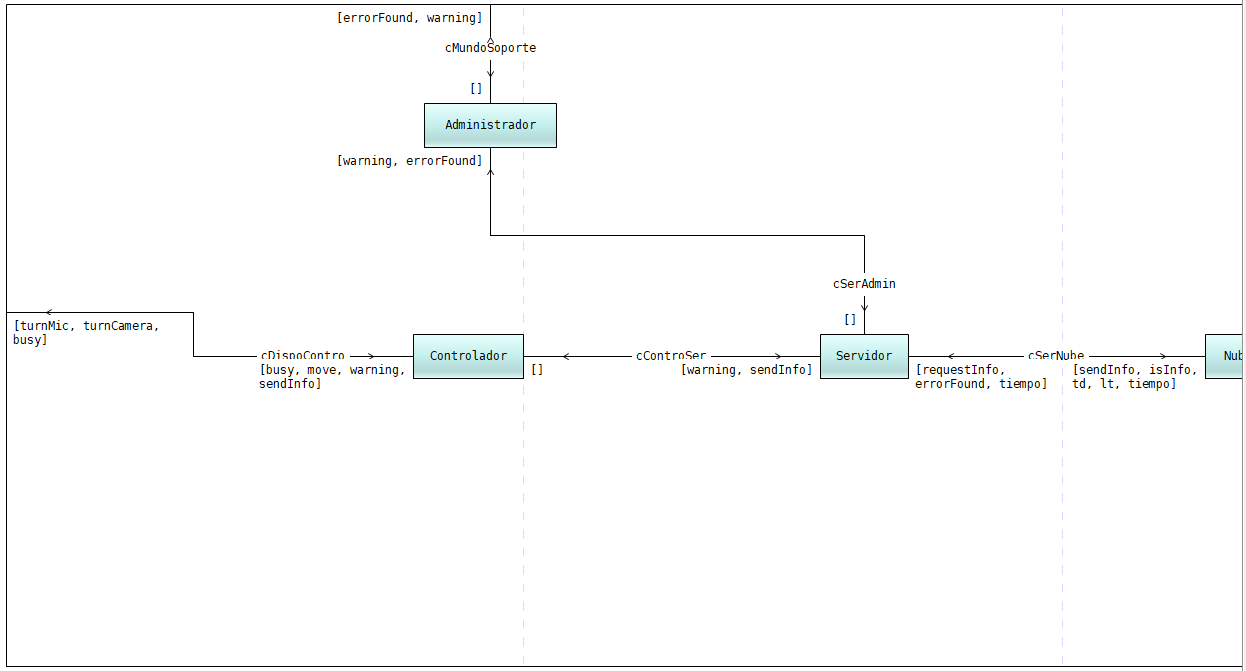
\includegraphics[width=0.7\textwidth]{images/Arquitectura_SDL1x.png}
    \caption{Diagrama SDL de la arquitectura general del sistema (1/2).}
    \label{ArquitecturaSDL1}
\end{figure}

En la figura \ref{ArquitecturaSDL2} se encuentra el resto de señales que salen de la nube a internet en general y es de donde también vienen las señales de los usuarios.

\begin{figure}[h]
    \centering
    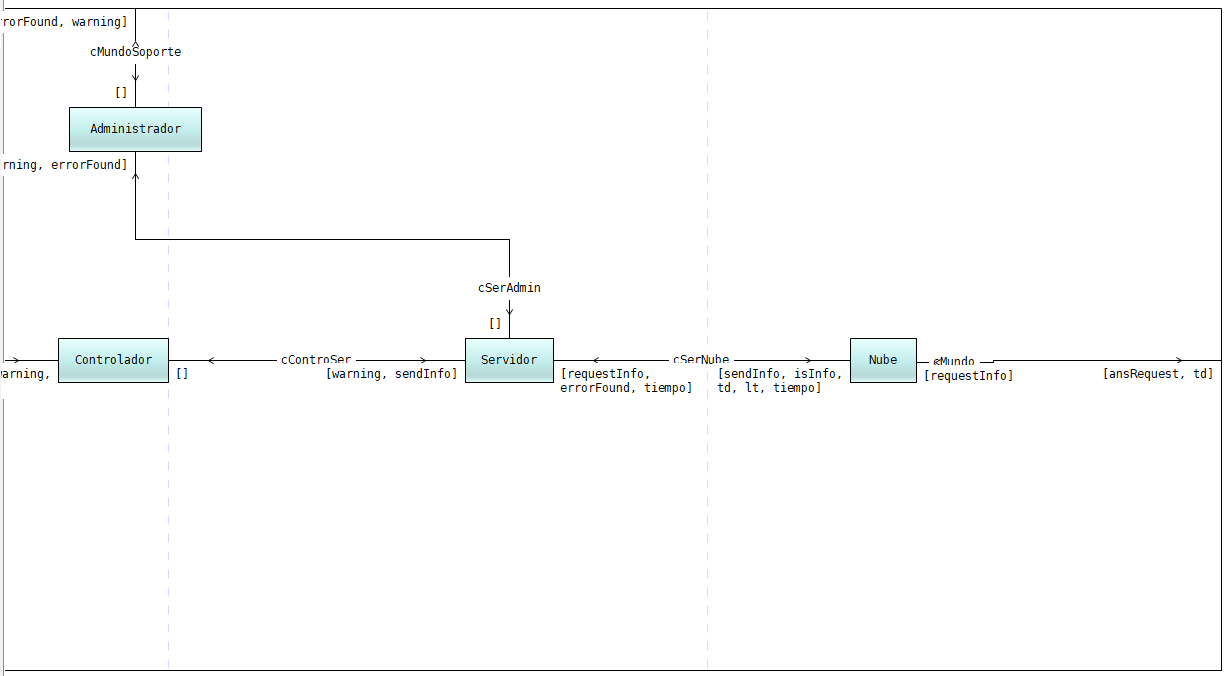
\includegraphics[width=0.7\textwidth]{images/Arquitectura_SDL2x.png}
    \caption{Diagrama SDL de la arquitectura general del sistema (2/2).}
    \label{ArquitecturaSDL2}
\end{figure}

\pagebreak

En la parte del controlador solo se encuentra el proceso que administra las entradas, salidas y los procedimientos que tiene como se puede ver en la figura \ref{ControladorSDL}.

\begin{figure}[h]
    \centering
    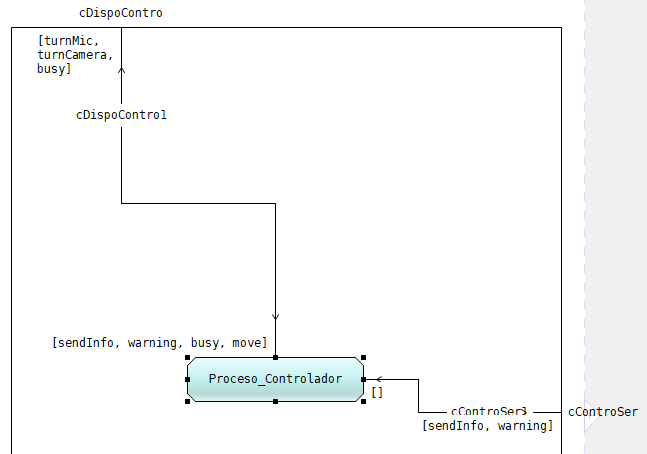
\includegraphics[width=0.7\textwidth]{images/Controladorx.png}
    \caption{Diagrama SDL del controlador.}
    \label{ControladorSDL}
\end{figure}

Dentro de dicho proceso se encuentra la máquina de estados de la figura \ref{ProcesoControladorSDL1}. Hubieron muchos cambios con respecto al modelo original, ya que se arreglaron errores del "sintaxis" y se consideraron más casos, juntando los procesos externos entre los dispositivos, el controlador y entre el controlador y el servidor, con al reducción de estos procesos en uno solo que maneja el controlador, refleja un buen comportamiento respecto al diagrama MSC que se estableció al principio.

\begin{figure}[h]
    \centering
    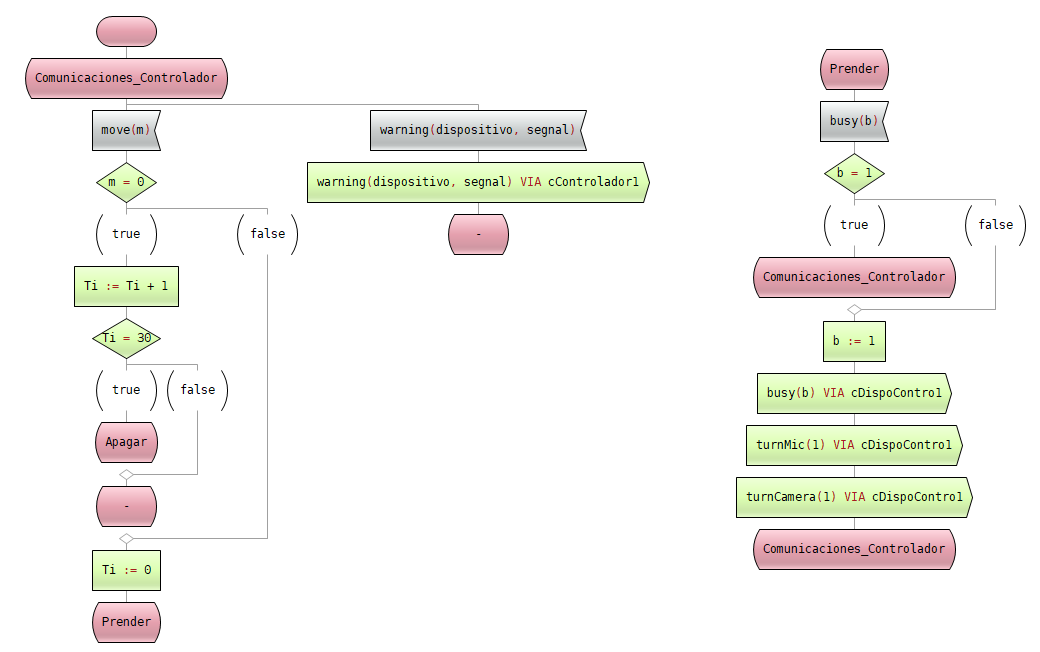
\includegraphics[width=0.8\textwidth]{images/Proceso_Controlador1x.png}
    \caption{Diagrama SDL del proceso del controlador (1/2).}
    \label{ProcesoControladorSDL1}
\end{figure}

\pagebreak

La otra parte de este proceso se muestra en la figura noc, sin embargo, es importante decir que no se están usando timers, sino tipos de variables que simulan temporizadores para medir el tiempo de como si fueran segundos con respecto al rango del movimiento registrado.

\begin{figure}[h]
    \centering
    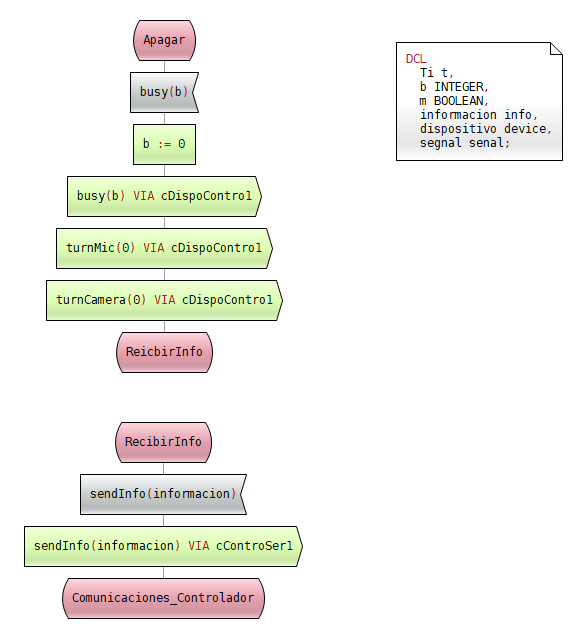
\includegraphics[width=0.4\textwidth]{images/Proceso_Controlador2x.png}
    \caption{Diagrama SDL del proceso del controlador (2/2).}
    \label{ProcesoControladorSDL2}
\end{figure}

\pagebreak

Ahora bien, en la parte del servidor no cambio nada, sigue estando igual al modelo principal dentro del servidor, lo único que cambia es el contenido del proceso dentro del servidor en la figura \ref{ServidorSDL1} y en la figura \ref{ServidorSDL2} .

\begin{figure}[h]
    \centering
    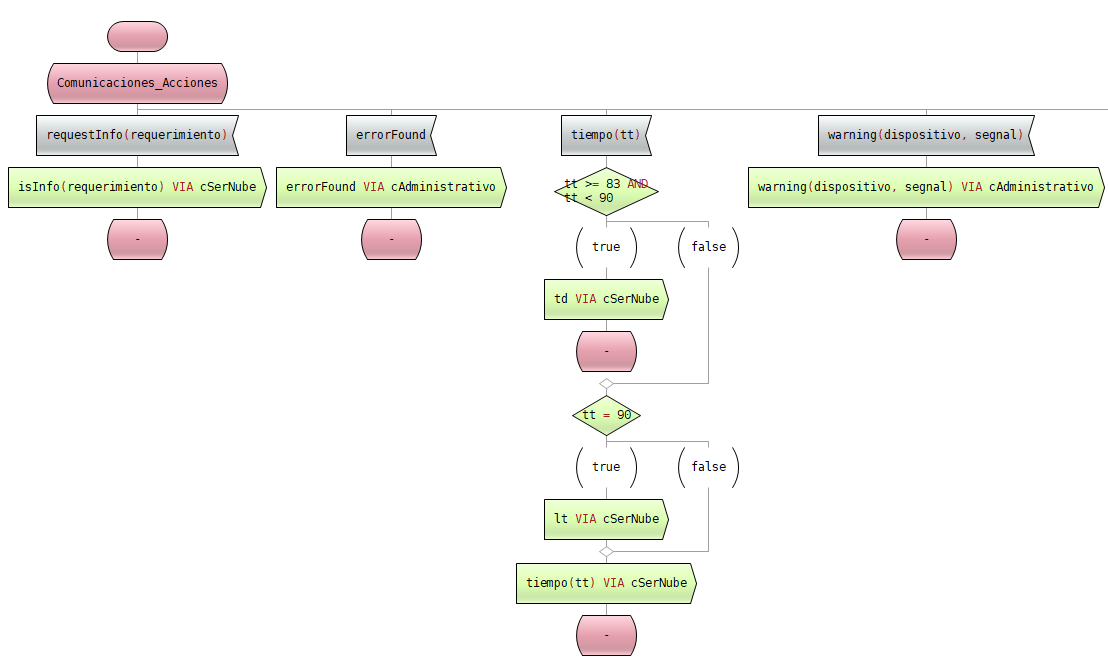
\includegraphics[width=0.9\textwidth]{images/Proceso_Servidor1x.png}
    \caption{Diagrama SDL del proceso del servidor (1/2).}
    \label{ServidorSDL1}
\end{figure}

De hecho, en la figura \ref{ServidorSDL2}, se ve como se usan dos estados de \emph{sendInfo} en los cuales el primero 

\begin{figure}[h]
    \centering
    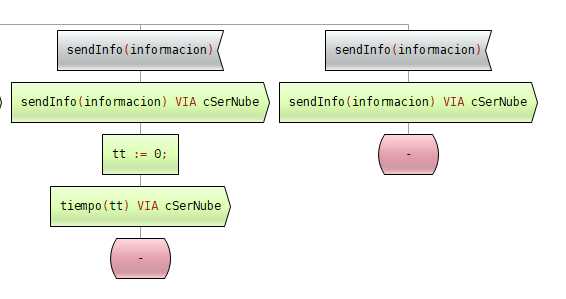
\includegraphics[width=0.6\textwidth]{images/Proceso_Servidor2x.png}
    \caption{Diagrama SDL del proceso del servidor (2/2).}
    \label{ServidorSDL2}
\end{figure}

\pagebreak

En la parte del administrador tampoco cambió, solo se redujeron procesos y se usó el mismo del planteamiento inicial de la arquitectura. Por otro lado la nube cambió ya que se incluyeron más cosas por el timer y se solucionaron otros errores en las entradas y salidas de los procesos. La arquitectura del servidor es la siguiente figura \ref{Nubex}.

\begin{figure}[h]
    \centering
    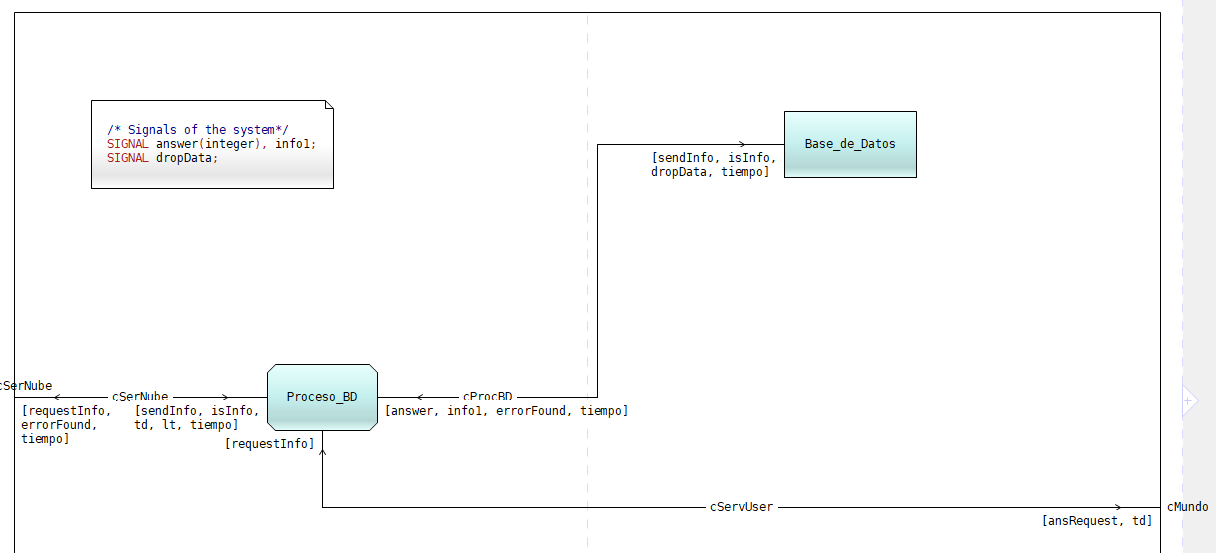
\includegraphics[width=1.0\textwidth]{images/Nubex.png}
    \caption{Diagrama SDL de la nube.}
    \label{Nubex}
\end{figure}

Dentro del proceso que conecta el servidor con la base de datos se ve lo siguiente en la figura \ref{ProcesoBD1}.

\begin{figure}[h]
    \centering
    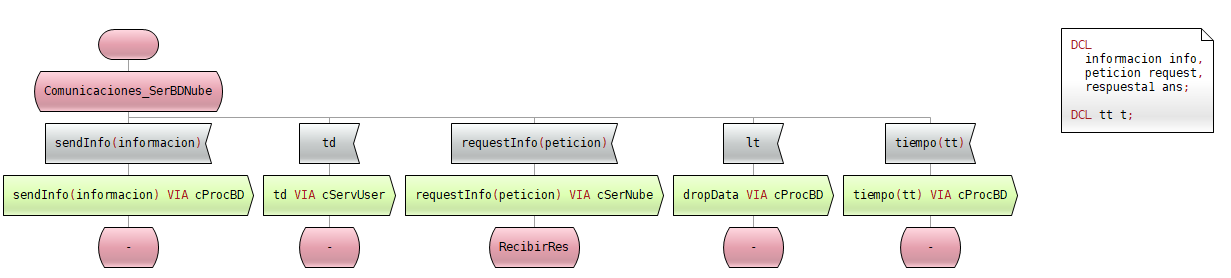
\includegraphics[width=1.0\textwidth]{images/Proceso_BD1x.png}
    \caption{Diagrama SDL del proceso que conecta la nube con el servidor (1/2).}
    \label{ProcesoBD1}
\end{figure}

Donde los estados para recibir las respuestas de la base de datos para enviarlos y distribuirlos dependiendo si son errores o información correcta obtenida del requerimiento. De hecho, para el usuario se devuelve un tipo de respuesta dependiendo si es un error o si es una consulta válida (la información solicitada), si hay un error se el devuelve al usuario el error y al servidor para redirigirlo al administrador, esto se ve en la figura \ref{ProcesoBD2}.

\begin{figure}[h]
    \centering
    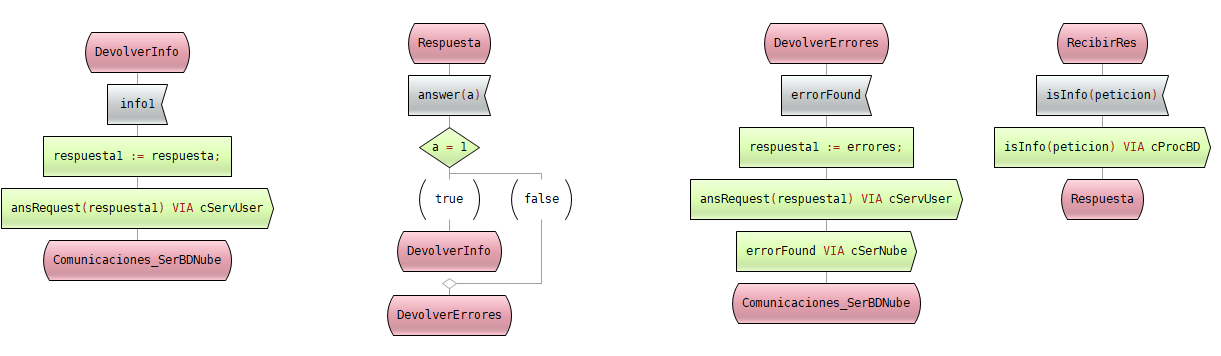
\includegraphics[width=1.0\textwidth]{images/Proceso_BD2x.png}
    \caption{Diagrama SDL del proceso que conecta la nube con el servidor (2/2).}
    \label{ProcesoBD2}
\end{figure}

\pagebreak

Por último, el proceso que maneja la base de datos se encarga de procesar el tiempo que se inicia desde el servidor y este lo suma y lo vuelve a enviar, esto con el propósito de revisar el tiempo en el servidor, realmente el manejo del tiempo se puede hacer en otro proceso, pero la decisión de elegir el proceso que hiciera esto fue arbitraria y sin preferencia, por decisión de los involucrado en el proyecto se escogió el proceso que maneja la base de datos, de hecho, una posible mejor es hacer un proceso que maneje la parte del tiempo internamente en el servidor. El proceso que gestiona la base de datos se puede ver en la figura \ref{ProcesoGestionBDSDL}.

\begin{figure}[h]
    \centering
    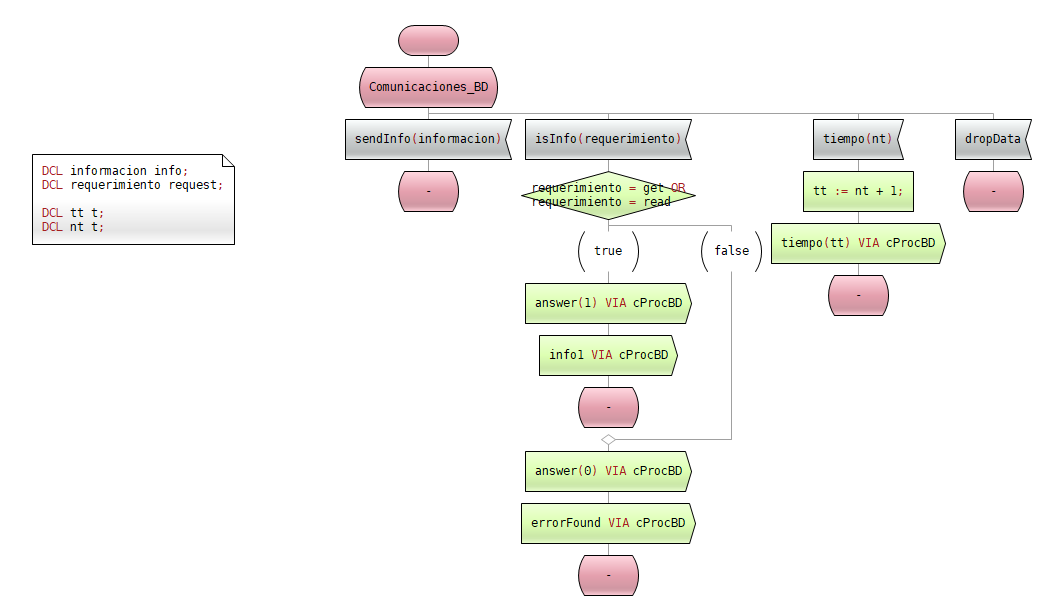
\includegraphics[width=0.85\textwidth]{images/Proceso_GestionBDx.png}
    \caption{Diagrama SDL del proceso que gestiona la base de datos.}
    \label{ProcesoGestionBDSDL}
\end{figure}

\pagebreak

Adicionalmente, se establecieron las declaraciones de las señales y los tipos de datos generales de la arquitectura en la figura \ref{DeclaracionesSDL}.

\begin{figure}[h]
    \centering
    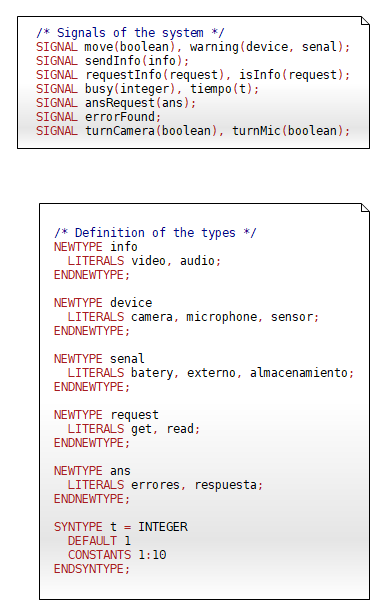
\includegraphics[width=0.5\textwidth]{images/Declaracionesx.png}
    \caption{Diagrama SDL de las declaraciones generales de la arquitectura.}
    \label{DeclaracionesSDL}
\end{figure}

\pagebreak

%%==================================================================================
\begin{comment}
    \section{Verificación del sistema escalado}
    
    Presente el plan de pruebas y los resultados de las diferentes pruebas realizadas al diseño (trazas de ejecución MSC) con los que se muestre la validez del diseño escalado frente a los requerimientos definidos previamente.
\end{comment}
%%==================================================================================
\begin{comment}
    \section{Implementación del sistema base}

    A partir del sistema base modelado en PragmaDev Studio, se construye un prototipo usando hilos (\href{https://en.wikipedia.org/wiki/Pthreads}{\textit{POSIX pthreads}}) en Linux con una única instancia por proceso SDL.\\
    
    Describa el proceso de implementación y el plan de pruebas (escenarios y casos de prueba)  del prototipo implementado (diagramas, modelos matemáticos, modelos a escala, montajes reales o “virtuales”, etc.). Incluya:
    
    \begin{itemize}
        \item Diagrama de despliegue
        \item Pruebas realizadas con usuarios
        \item Aprendizajes obtenidos
    \end{itemize}
\end{comment}
